\documentclass[a4paper,twoside]{memoir}
% Set up encoding
\usepackage[utf8]{inputenc}

% Mulighed for at definere acronyms
\usepackage{acronym}

% Load up bibliography.
\usepackage[authoryear]{natbib}
\setcitestyle{numbers,square}
% Bibliography style.
\bibliographystyle{plainnat}

% Algorithm support.
\usepackage{algorithmic}
\usepackage{algorithm}
\usepackage{subfig}
\usepackage{amsmath}
\usepackage{amsfonts}
% Make algorithms appear as procedures instead.
\floatname{algorithm}{Procedure}
\renewcommand{\algorithmicrequire}{\textbf{Input:}}
\renewcommand{\algorithmicensure}{\textbf{Output:}}

% Image frames.
\setlength{\fboxsep}{0pt}
\setlength{\fboxrule}{0.5pt}

% Also, images.
\usepackage{graphicx}

% tabeller der strækker sig over flere sider
\usepackage{longtable}

% flere tabel-muligheder
\usepackage{multirow}

% bedre enumerate
\usepackage{enumitem}

% Todo notes here and there.
% write instead for disable: \usepackage[disable]{todonotes}
\usepackage{todonotes}

% Forbedrede floats.
\usepackage{float}
\usepackage{rotating}

% Special symbols availability.
\usepackage{amssymb}

%Degree symbol
\usepackage{gensymb}

% Wrap figure
\usepackage{wrapfig}

%landscape mode
\usepackage{lscape}

%Fun with captions
\usepackage{caption}

% Operationel semantik
\newcommand{\lag}{\langle}
\newcommand{\rag}{\rangle}
\newcommand{\setof}[2]{\ensuremath{\{ #1 \mid #2 \}}}
\newcommand{\set}[1]{\ensuremath{\{ #1 \}}}
\newcommand{\besk}[1]{\ensuremath{\lag #1 \rag}}
\newcommand{\ra}{\rightarrow}
\newcommand{\lra}{\longrightarrow}
\newcommand{\Ra}{\Rightarrow}

% CODE %
\usepackage{listings}
\usepackage{color}
%\usepackage{bera}
\definecolor{gray}{rgb}{0.4,0.4,0.4}
\definecolor{darkblue}{rgb}{0.0,0.0,0.6}
\definecolor{cyan}{rgb}{0.0,0.6,0.6}
\lstset{
  basicstyle=\ttfamily,
  columns=fullflexible,
  showstringspaces=false,
  commentstyle=\color{gray}\upshape,
  basicstyle=\small,
  numberstyle=\footnotesize,
  numbers=left,
  captionpos=b,
  stepnumber=1,
  numbersep=10pt,
  tabsize=2,
  breaklines=true,
}
% Define markup of XML
\lstdefinelanguage{XML}
{
  morestring=[b]",
  morestring=[s]{>}{<},
  morecomment=[s]{<?}{?>},
  identifierstyle=\color{darkblue},
  keywordstyle=\color{cyan},
  morekeywords={id, target, type, category, value, point, correct, rows, width, time}% list your attributes here
}
% Define markup of C#
\lstdefinelanguage{CSharp}[Visual]{C++}
{
	identifierstyle=\color{darkblue},
	commentstyle=\color{green!70!black}\itshape ,
	stringstyle=\color{gray},
	sensitive=true,
	morestring=[b]",
	morestring=[b]',
	morecomment=[l]//,
	morecomment=[n]{/*}{*/}
}

% Define markup of Javascript
\lstdefinelanguage{JavaScript}{
  keywords={typeof, new, true, false, catch, function, return, null, catch, switch, var, if, in, while, do, else, case, break},
  keywordstyle=\color{blue}\bfseries,
  ndkeywords={class, export, boolean, throw, implements, import, this},
  ndkeywordstyle=\color{darkgray}\bfseries,
  identifierstyle=\color{black},
  sensitive=false,
  comment=[l]{//},
  morecomment=[s]{/*}{*/},
  commentstyle=\color{purple}\ttfamily,
  stringstyle=\color{red}\ttfamily,
  morestring=[b]',
  morestring=[b]"
}

% Define markup of JSON
\colorlet{punct}{red!60!black}
\definecolor{background}{HTML}{EEEEEE}
\definecolor{delim}{RGB}{20,105,176}
\colorlet{numb}{magenta!60!black}
\lstdefinelanguage{json}{
    basicstyle=\normalfont\ttfamily,
    numbers=left,
    numberstyle=\scriptsize,
    stepnumber=1,
    numbersep=8pt,
    showstringspaces=false,
    breaklines=true,
    frame=lines,
    backgroundcolor=\color{background},
    literate=
     *{0}{{{\color{numb}0}}}{1}
      {1}{{{\color{numb}1}}}{1}
      {2}{{{\color{numb}2}}}{1}
      {3}{{{\color{numb}3}}}{1}
      {4}{{{\color{numb}4}}}{1}
      {5}{{{\color{numb}5}}}{1}
      {6}{{{\color{numb}6}}}{1}
      {7}{{{\color{numb}7}}}{1}
      {8}{{{\color{numb}8}}}{1}
      {9}{{{\color{numb}9}}}{1}
      {:}{{{\color{punct}{:}}}}{1}
      {,}{{{\color{punct}{,}}}}{1}
      {\{}{{{\color{delim}{\{}}}}{1}
      {\}}{{{\color{delim}{\}}}}}{1}
      {[}{{{\color{delim}{[}}}}{1}
      {]}{{{\color{delim}{]}}}}{1},
}

\lstdefinelanguage{KAPAOOW}{
 sensitive=false,
 keywords={character, characters, action, end, if, then, else, from, to, downto, next, while, loop, use, turn, begins, ends, select, wins, draw, random, of, case, cases, enemy, player, start, skip, attack, types, damage, defend, by, using, message, and, or, is, value, mod},
 identifierstyle=\itshape,
 keywordstyle=\bfseries,
 stringstyle=\normalfont,
 morestring=[b]",
 comment=[l]{//},
 commentstyle=\color{gray}
}

% Neat-o referencer...o.
\usepackage{bookmark,hyperref}
\usepackage{nameref}

% hack fra nettet.
% http://tex.stackexchange.com/questions/1230/reference-name-of-description-list-item-in-latex
\makeatletter
\let\orgdescriptionlabel\descriptionlabel
\renewcommand*{\descriptionlabel}[1]{
  \let\orglabel\label
  \let\label\@gobble
  \phantomsection
  \edef\@currentlabel{#1}
  %\edef\@currentlabelname{#1}
%  \let\label\orglabel
  \orgdescriptionlabel{#1}
}
\makeatother
% Rettehak. Meget lettere end \checkmark
\newcommand{\yes}{\checkmark}


% Create a new command, HRule, to insert some nice horisontal rules on the title page.
\newcommand{\HRule}{\rule{\linewidth}{0.3mm}}

% New command for two figures, side by side.
\newcommand{\twofigs}[6]
{
	\begin{figure}[H]
		\begin{minipage}[b]{0.5\columnwidth}
		\centering
		\includegraphics[width=0.8\columnwidth]{img/#1}
		\caption{#2\label{#3}}
		\end{minipage}
		\hspace{0.5cm}
		\begin{minipage}[b]{0.5\columnwidth}
		\centering
		\includegraphics[width=0.8\columnwidth]{img/#4}
		\caption{#5\label{#6}}
		\end{minipage}
	\end{figure}
}

% Sørg for at paragrafplads ikke spildes.
\raggedbottom

% Package til at regne forskellen ud mellem 2 labels
\usepackage{refcount}
\newcommand{\pagedifference}[2]{\number\numexpr\getpagerefnumber{#2}+1-\getpagerefnumber{#1}\relax}

\usepackage{color,calc,graphicx,soul,fourier}
\definecolor{aaublue}{RGB}{33,26,82}
\makeatletter
\newlength\dlf@normtxtw
\setlength\dlf@normtxtw{\textwidth}
\def\myhelvetfont{\def\sfdefault{mdput}}
\newsavebox{\feline@chapter}
\newcommand\feline@chapter@marker[1][4cm]{%
  \sbox\feline@chapter{%
    \resizebox{!}{#1}{\fboxsep=1pt%
      \colorbox{aaublue}{\color{white}\bfseries\sffamily\thechapter}%
    }}%
  \rotatebox{90}{%
    \resizebox{%
      \heightof{\usebox{\feline@chapter}}+\depthof{\usebox{\feline@chapter}}}%
    {!}{\scshape\so\@chapapp}}\quad%
  \raisebox{\depthof{\usebox{\feline@chapter}}}{\usebox{\feline@chapter}}%
}
\newcommand\feline@chm[1][4cm]{%
  \sbox\feline@chapter{\feline@chapter@marker[#1]}%
  \makebox[0pt][l]{% aka \rlap
    \makebox[1cm][r]{\usebox\feline@chapter}%
  }}
\makechapterstyle{daleif1}{
  \renewcommand\chapnamefont{\normalfont\Large\scshape\raggedleft\so}
  \renewcommand\chaptitlefont{\normalfont\huge\bfseries\scshape\color{aaublue}}
  \renewcommand\chapternamenum{}
  \renewcommand\printchaptername{}
  \renewcommand\printchapternum{\null\hfill\feline@chm[2.5cm]\par}
  \renewcommand\afterchapternum{\par\vskip\midchapskip}
  \renewcommand\printchaptertitle[1]{\chaptitlefont\raggedleft ##1\par}
}
\makeatother
\chapterstyle{daleif1}
\setlength\afterchapskip {\onelineskip }
\setlength\beforechapskip {\onelineskip }
\usepackage{lipsum}


\acrodef{api}[API]{Application Programming Interface}
\acrodef{cat}[CAT]{Category Adminitration Tool}
\acrodef{lamp}[LAMP]{Linux, Apache2, MySql and PHP}
\acrodef{giraf}[GIRAF]{Graphical Interface Resources for Autistic Folk}
\acrodef{oha}[OHA]{Open Handset Alliance}
\acrodef{gui}[GUI]{Graphical User Interface}
\acrodef{json}[JSON]{JavaScript Object Notation}

\acrodef{opengles}[OpenGL ES]{OpenGL for Embedded Systems}
\acrodef{pot}[POT]{power-of-two}
\acrodef{npot}[NPOT]{non-power-of-two}
\acrodef{3d}[3D]{Three-dimensional space}
\acrodef{2d}[2D]{Two-dimensional space}

\begin{document}

\begin{titlingpage}
\begin{center}
% Upper part of the page. The '~' is needed because \\
% only works if a paragraph has started.

\includegraphics[width=0.30\textwidth]{img/titelblad/AAU_logo_2012}~\\[0.5cm]

\textsc{\LARGE Aalborg University}\\[0.3cm]

\textsc{\Large Bachelor project}\\[0.5cm]

% Title
\HRule \\[0.4cm]
{ \huge \bfseries Train}\\[0.3cm]
{ \bfseries Optional subtitle}

\HRule \\[0.4cm]

% Author and supervisor
\begin{minipage}{\textwidth}
\begin{center}
	Aalborg University, Department of Computer Science\\
	P6, Spring semester 2013\\
	Project group sw606f13 / 5.1.38\\
\end{center}
\end{minipage}\\[1cm]

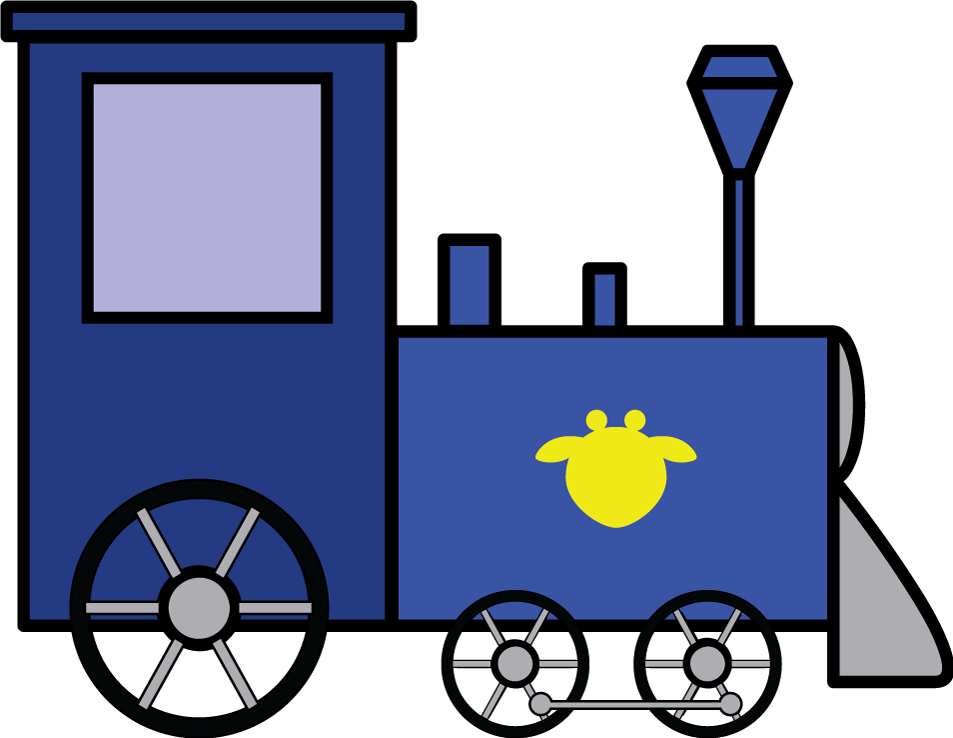
\includegraphics[width=\textwidth]{img/train}

\vfill



% Bottom of the page
{\large \today}

\end{center}
\end{titlingpage}


\newpage
\thispagestyle{empty}
\mbox{}

\newpage
\thispagestyle{empty}
\mbox{}

\thispagestyle{empty}
\begin{titlepage}
\begin{nopagebreak}
\setcounter{page}{3}
{\samepage 
\begin{tabular}{r}
\parbox{\textwidth}{  \raisebox{11mm}{
\includegraphics[height=1.2cm]{img/Titelblad/logo.jpg}}
\hfill \parbox{4.9cm}{\begin{tabular}{l}
{\sf\small \textbf{Department of Computer Science }}\\
{\sf\small  \textbf{Software Engineering}} \\
{\sf\small Selma Lagerløfs Vej 300} \\
{\sf\small Telephone +45 9940 9940} \\
{\sf\small +45 9940 9798} \\
{\sf\small http://www.cs.aau.dk}
\end{tabular}}}
\\
\end{tabular}

\begin{tabular}{cc}
\parbox{6cm}{
\begin{description}

\item {\bf Title:} 

Train
  
\item {\bf Subject:} 
Developing Complex Software Systems.

\end{description}

\parbox{8cm}{

\begin{description}
\item {\bf Project period:}\\
   P6, Spring semester 2013\\
  \hspace{4cm}
\item {\bf Project group:}\\
  SW606f13\\
  \hspace{4cm}
\item {\bf Attendees:}\\
Jacob Karstensen Wortmann \\
Jesper Riemer Andersen \\
Nicklas Andersen \\
Simon Reedtz Olesen \\

  \hspace{2cm}
\item {\bf Supervisor:}\\
Ulrik Mathias Nyman \\
\end{description}
}
\begin{description}
\item {\bf Finished:}
\item {\bf Number of pages:} \pageref{lastpage}
\item {\bf Appendix pages:} \pagedifference{appendixStart}{appendixEnd}
\end{description}
\vfill } &
\parbox{7cm}{
  \vspace{.15cm}
  \hfill 
  \begin{tabular}{l}
  {\bf Synopsis:}\bigskip \\
  \fbox{
    \parbox{6.5cm}{\bigskip
     {\vfill{\small %blank
     \bigskip}}
     }}
   \end{tabular}}
\end{tabular}}
\\ \\
\noindent{\footnotesize\emph{The content of this rapport can be used freely; however publication (with source material) may only occur in agreement with
the authors.}}
\end{nopagebreak}
\end{titlepage}
% Titelblad

\chapter*{Signatures}
\setcounter{page}{7}
\thispagestyle{empty}

\noindent\rule{8cm}{0.03cm}\\
Jacob Karstensen Wortmann\\\\

\noindent\rule{8cm}{0.03cm}\\ 
Jesper Riemer Andersen\\ \\

\noindent\rule{8cm}{0.03cm}\\
Nicklas Andersen\\\\

\noindent\rule{8cm}{0.03cm}\\
Simon Reedtz Olesen\\\\


\newpage
\thispagestyle{empty}
\mbox{}

\chapter*{Preface}
This project was written as the Bachelor project by group SW606F13 - Software students from the Department of Computer Science at Aalborg University in the spring of 2013. The report documents the GIRAF project of 2013 and the implementation of the Train application. The application is developed for the Android platform. The reader is expected to be familiar with Java and UML. We have included our knowledge from all our previous semesters.
\\\\
When reading the report, there are a few things the reader should be aware of:
\begin{itemize}
\item When a reference to a source of a section or paragraph is given, the number of the source is written inside square brackets $[\;]$. The number is a reference to the bibliography list on page \pageref{chap:bib}.
\item When "we/us/our" is mentioned in the report, it is a referral to the authors of the report
\end{itemize}
We would like to thank our supervisor Ulrik Mathias Nyman for the feedback he has given throughout the project.


\newpage
\thispagestyle{empty}
\mbox{}

\newpage
\thispagestyle{empty}
\mbox{}

\setcounter{secnumdepth}{3}
\setcounter{tocdepth}{1}

\tableofcontents

\newcommand{\secref}[1]{Section \ref{#1}} %brugt i fællesrapporten

\chapter{Introduction}\label{chap:intro}

\section*{Project introduction}
We implement a game for children with autism on the Android platform, as a part of the GIRAF project.

The inspiration for our game comes from an exercise one of the pedagogues practises with the children. The purpose of the game is to create a dialogue between the child and the pedagogue. The child has to drag pictograms from a train station onto the train wagons and make the train drive. When the train arrives at the next station, the child has to drag the correct pictograms from the train and onto the station. The correct pictograms are decided by the station
category.

The category for each station is chosen by the pedagogues by clicking the category picture frame and browse the pictogram database and choose the picture they want to use. After selecting a category they select which pictures they want associated with this station, these are the pictograms the children have to drag onto this specific station.

\subsection*{Problem Statement}
Based on our focus in the multiproject, we have come up with the following problem statement:
In what ways can we aid the pedagogues in their work, with children with autism, by digitalizing a physical exercise onto an Android tablet?

\input{tex/commonReport/commonReport.tex}

\chapter{Chronological process} \label{chronologicalprocess}
\chapter{Chronological process}
\label{chronologicalprocess}

\todo{This Chapter describes the process of developing our game. At the end of each week, we wrote down what we had done and what choices we had made.}

\section*{Week 1 - 18/02/2013 - 22/02/2013}

After forming our groups we spent the first week brainstorming for ideas for a game. We had our first supervisor meeting this week as well, where we presented our initial idea and got some feedback, which we used as input. 

\section*{Week 2 - 18/02/2013 - 22/02/2013} 
\label{processweek2}
After some brainstorming and discussions with our supervisor we came up with an idea for our game, the game idea takes base in Tove's own exercise with the children. In one of the introduction weeks of this semester, Tove presented how she works with the children, improving their communication, categorization of objects, and social skills. In one of her exercises she try to improve the child's skill to categorize objects. This exercise consist of making the child take the right object, placing it on a train, and drive the train to the correct train station that accepts this object. This exercise has proven to Tove to be very powerful since it can be modified to help children categorize colors, sizes of objects, people of the child's social circle, and more. Though the exercise is good, the preparation time for each game can be very time consuming. She often has to make new pictograms or find objects of a certain requirements. Our game idea is to digitize the exercise and keep the principles of the exercises, by moving the exercise to a tablet, we also hope that the preparation time for each child is reduced.

When the general game idea was agreed upon, we began developing and designing the interface. The interface should be simple and its main functionality should be to drag and drop pictograms on and off the train. We created a simple paper prototype of the design.

We arranged a meeting with Tove, so that we could present our idea and show her the paper prototype that we made to demonstrate our idea. The feedback we received was used throughout the project to design our game.\todo{måske skriv resultatet af mødet her i stedet for i sec: design - game}

Since this is a project that we are continuing from last year we had to set up Eclipse so that we could compile the old projects and run them on our tablet. 

After setting up Eclipse we spent the rest of the time experimenting with Android code and make small runnable programs. 

\section*{Week 3 - 25/02/2013 - 01/03/2013}

We are now able to drag and drop pictograms to different boxes. In case a box is already filled, then the dragged picture snaps back to its original box. In case you release the pictogram outside a box it will snap back to its original box. 

We also discussed how the layout of our game should be, in regards to where each pictogram box, train station, train etc. should be. 

We also looked into different methods to make our background slide to create the illusion that our train was moving between stations. 

\section*{Week 4 - 04/03/2013 - 08/03/2013}
We now had a sliding background which worked, however we discovered that it was too slow, so we instead had a discussing of whether or not we should use OpenGL. 

We also started making the graphics we needed for our game, using Adobe Illustrator.\todo{Kan man refere til design komiten?} We wanted to draw all the graphics in vector graphics so that we could easily scale it up or down without losing quality. 

We also had a short discussing regarding how to make it look like the train was moving. 

\section*{Week 5 - 11/03/2013 - 15/03/2013}
This week we finished Sprint 1, which focused on getting our application into the existing GIRAF launcher. We achieved this. 

We were also asked, by the Chief Integration Officer (\textbf{CIO} to make an ant script for our project so that he could set up continues integration for the multiproject. This was also achieved. 

We have decided to use OpenGL, since the alternative was way too slow. We use OpenGL to render our graphics. We are able to draw objects / pictures on the screen using OpenGL. 

We also created a little icon for our game. 

We had the second meeting with Tove this week as well, she gave some comments on our graphic and us some great ideas for improvement that we can use. She also suggested that there could be changing weather when the train moved from station to station. 

\section*{Week 6, 7, 8 and 9 - 18/03/2013-12/04/2013}
Since the last notes we have done a lot of "under the hood" work:

\begin{itemize}
\item We have decided to use OpenGL ES V1 instead of the newer V2. We chose to use V1 because it should be easier for OpenGL beginners. 
\item The class diagram (structure) for OpenGL drawing is implemented. It is now easy to draw and move objects across the screen. 
\item The wheels on the train and the smoke coming from the exhaust is now animated to create the illusion that the train is actually moving. 
\item The train can now smoothly accelerate and decelerate and can stop at exact coordinates in front of a station. 
\item "Garbage" has been improved, Garbage collection does almost not run any more. 
\item We have implemented the Pictogram class.
\item We sent an e-mail to Tove with some prototypes of how the game looks. She has replied with some improvement.
\end{itemize} 

\section*{Week 10, 11, 12 and 13 - 12/04/2013 - 10/05/2013}
Since the last notes we have almost finished the game, just need to fix a few bugs. Among the things we have implemented are:

\begin{itemize}
\item We now have hills in the background. They are made in sequences of four hills and are randomly picked throughout the game. 
\item We now have clouds and a sun on the sky. The clouds are moving at a random speed and at a random height on the sky. 
\item We now have cows and trees on the hills. These come at random times throughout the game.
\item We now have a train depot to indicate that the game has finished. 
\todo{Vi skal lige have skrevet alt på og have skrevet at vi har afsluttet hvert sprint.}
\end{itemize}
We also started writing on our report. 

\section*{Week 14 - 13/05/2013 - 17/05/2013}
\todo{Skrive noter}
\section*{Week 15 - 20/05/2013 - 24/05/2013}
\todo{Skrive noter} 


\chapter{Android}
\todo{This Chapter describes the Android platform, and which functionality of the Android platform that we have used.}



OpenGL is a 2D and 3D graphics API. It is a cross-platform API that specifies a standard for 3D graphics processing hardware. Android $1.0$ and later versions have support for \ac{opengles} $1.0$ and $1.1$ specifications. Android $2.2$ added support for \ac{opengles} $2.0$. \citep{androidopengl, khronosopengles}

\subsubsection*{Choice of \ac{opengles} Version}
When using \ac{opengles} on the Android platform, the default \ac{opengles} version is $1.x$. If you want to use version $2.0$ you need to explicitly write that you are using it. Version $2.0$ should have better performance and more possibilities than the older version, but the Android developers guide says:
\begin{quote}
\textit{"Developers who are new to OpenGL may find coding for \ac{opengles} 1.0/1.1 faster and more convenient."} \citep{androidopengl}
\end{quote}
Since we are beginners to OpenGL we have chosen version $1.x$. One big difference between $1.x$ and $2.0$ is that you have to write your own shaders in versions $2.0$, this allows for easier effects customization. The Train game does not really require much special effects other than simple drawing of textures.

\section{Design}

In this section we show how we use \ac{opengles} to draw on the screen. The design description gets very close to an implementation description, but a few specific methods will be described in more detail in the next section.

\subsection{Renderable Classes}

Considering the game and its purpose, we came up with different objects that should be rendered. \autoref{fig:renderables} shows a simplified version of the different objects/classes that can be rendered. We needed to draw texture at different positions on the screen and we needed to be able to move texture around on the screen. This is the general idea and based on this, the following classes were created.

\begin{figure}[H]
\centering
\includegraphics[page=2,width=1\linewidth]{img/opengl.pdf}
\caption{Class diagram of the objects that can be rendered.}
\label{fig:renderables}
\end{figure}

\begin{description}
\item[Coordination/Renderable:] In order to move objects around we have the abstract super class \lstinline|Coordination| which defines the methods to move. The abstract class \lstinline|Renderable| specifies that the objects needed to be rendered on the screen must implement the abstract methods: \lstinline|draw()|, \lstinline|getWidth()|, and \lstinline|getHeight()|. If some \lstinline|Renderable| object has to be be drawn more than once, then instead of making two identical \lstinline|Renderable| objects with different coordinates, we have a list of coordinates in \lstinline|Coordination|. The \lstinline|move| method will then move all the coordinates by the specified amount. It was also a possibility to move only one specific coordinate by the specified amount, but this last scenario was never needed.

\item[RenderableMatrix:] Since almost everything is moved relative to the train's speed we needed some kind of grouping of \lstinline|Renderable| objects, that were moved together. This is what \lstinline|RenderableMatrix| handles. It is possible to add other \lstinline|Renderable| objects to the \lstinline|RenderableMatrix|, this means that it is also possible to add matrices to\todo{To rendablesmatrices?} matrices. The \lstinline|addRenderMatrixItem()| method also has a color as parameter to use when drawing the \lstinline|Renderable|, this parameter is not shown on the figure to reduce the size of it. When calling \lstinline|draw()| on this class, it iterates through all \lstinline|matrixItems| and calls draw on them. The \lstinline|draw()| method's color parameter for the \lstinline|RenderableMatrix| is ignored, and instead it uses the color specified for each matrix item.

The \lstinline|RenderableMatrix| must also implement the abstract methods \lstinline|getWidth()| and \lstinline|getHeight()|. The width is calculated by the difference between the lowest x-coordinate to the greatest x-coordinate, and the same goes for the height with the y-coordinate instead. This feature was used at the time when this was designed, but has later become unnecessary.

The \lstinline|RenderableMatrix| is made with a new OpenGL matrix, this will be explained in more detail in \secref{sec:gamerendering}.

\item[Shape:] Everything that takes the form of a shape e.g. a square or a triangle, must inherit from the abstract class \lstinline|Shape|. All shapes consists of an array of vertices. The vertices for the \lstinline|Shape| determines how it is drawn relative to the coordinate.

Since we need wheels to rotate on the train, \lstinline|Shape| implements a method to rotate the \lstinline|Shape| around its center.

\item[Square:] The \lstinline|Square| is initialised with a size in the constructor, and then vertices are created according to the specified size. We decided that the \lstinline|Square| should be drawn from the top-left corner on its coordinates.

The color in the \lstinline|draw()| method's parameter specify the color of the square.

\item[GradientSquare:] This is similar to the \lstinline|Square|, instead this square is initialised with two colors to create either a horizontal or a vertical color gradient between the two colors.

\item[Texture:] This is the most important and most used class when creating our game. Since all pictures/images are 'square', it inherits from \lstinline|Square|, and then the texture is mapped onto that \lstinline|Square|.

This class must at some point load a resource pointer to a texture pointer. The loaded texture will always stretch to the size of the \lstinline|Square| that it is drawn upon. The \lstinline|Texture| class also implements ways to keep the original aspect ratio of the texture. Although not shown in the figure, the \lstinline|loadTexture()| method also has an aspect ratio option that allows the size of the \lstinline|Square|, containing the texture, to resize based on the size of the texture.

During loading of a piece of texture, the texture is converted to a \ac{pot} sized texture, \secref{sec:potsupport} explains why. \ac{opengles} has maximum dimensions for texture which is dependent on the device in use \citep{glutils}. Each piece of texture is checked whether they respect the maximum dimensions, if it does not it is scaled down.

The \lstinline|draw()| method must be overridden in order to draw the loaded texture. In this case it is possible to change the color that the \lstinline|Texture| is drawn with. No matter what color the original \lstinline|Texture| is, a color filter can be put on top of that on each call of the draw method.

\item[Text:] Adds the possibility to draw text. \lstinline|loadText()| generates a bitmap with the specified text to use as texture. This is an easy way to draw text, but if you need to draw text that changes all the time, then \lstinline|loadText()| is a slow way to do it. Fortunately we only need to load one time for each \lstinline|Text| object.

\item[GlPictogram:] Adds the possibility to draw a pictogram. The method \lstinline|loadPictogram()| generates a bitmap of the pictogram image, and then uses it as the texture for the object. To draw the pictogram text, a \lstinline|Text| object is used.
\end{description}

\subsection{Texture Power-of-two Support}\label{sec:potsupport}
Some \ac{opengles} devices does not support texture with a \ac{npot} size, they only accept texture with a \ac{pot} size, i.e. $2^x$. Android developers reference states that you should perform a check whether the current context supports \ac{npot}. \citep{glutils}

You get an increase of performance when using \ac{pot}, and at the time when the first version of OpenGL was created, the hardware needed this extra performance. Years later hardware only gained an insignificant increase of performance so they allowed \ac{npot}. Some embedded systems using \ac{opengles} still gain a significant increase in performance, and this is why some devices require texture to be \ac{pot}. (We were not able to find official citation, the best we could find is this \citep{potperformance})

Instead of performing a check to see whether the current context supports \ac{npot}, we choose to always use \ac{pot}. Even if it is not necessary it will still give a small performance increase. The way we achieve this is to still use texture with a \ac{npot} size, convert the texture to \ac{pot} size, and then stretch it relative to the change in size. However this will also consume a lot more memory, but the train game does not require that much memory even with \ac{pot} sized texture.
\begin{figure}[H]
\begin{minipage}[b]{0.5\columnwidth}
\centering
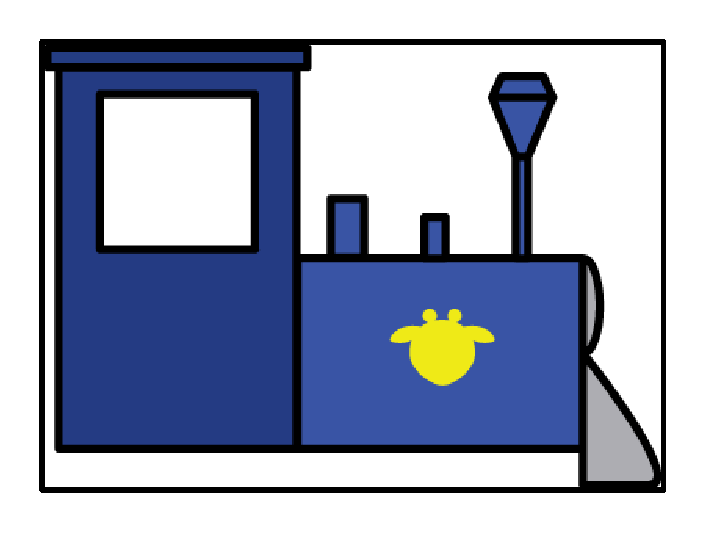
\includegraphics[page=1,width=0.8\columnwidth]{img/powerOfTwo.pdf}
\caption{The \ac{npot} train texture inside the \lstinline|Square| container.\label{fig:train}}
\end{minipage}
\hspace{0.5cm}
\begin{minipage}[b]{0.5\columnwidth}
\centering
\includegraphics[page=2,width=0.8\columnwidth]{img/powerOfTwo.pdf}
\caption{The \ac{pot} train texture.\label{fig:trainpot}}
\end{minipage}
\end{figure}
\autoref{fig:train} shows the train texture inside the \lstinline|Square| container. The black line illustrates the \lstinline|Square|, this is shown for the sake of the example and it is of course not shown in the actual application. The texture has a size of $396 \times 284$ pixels, and need to be converted to a \ac{pot} size.

\autoref{fig:trainpot} shows the train texture with alpha channels to the right and below the texture to obtain a \ac{pot} texture with the size of $512 \times 512$ pixels.
\begin{figure}[H]
\begin{minipage}[b]{0.5\columnwidth}
\centering
\includegraphics[page=3,width=0.8\columnwidth]{img/powerOfTwo.pdf}
\caption{The \ac{pot} train texture inside the \lstinline|Square| container.\label{fig:trainneedcrop}}
\end{minipage}
\hspace{0.5cm}
\begin{minipage}[b]{0.5\columnwidth}
\centering
\includegraphics[page=4,width=0.8\columnwidth]{img/powerOfTwo.pdf}
\caption{The \ac{pot} train texture after stretching.\label{fig:trainresult}}
\end{minipage}
\end{figure}
When we take the new \ac{pot} sized texture and insert it into the \lstinline|Square| the texture will still clamp to the edges. \autoref{fig:trainneedcrop} shows the clamped train texture.

We need to adjust the texture in order to fit the \ac{pot} texture inside the \lstinline|Square|. We stretch the texture by mapping the texture outside of the \lstinline|Square| relative to the change in size from \ac{npot} to \ac{pot}. Since nothing outside the borders of the \lstinline|Square| is drawn, then you could also say that the extra alpha channels are cropped away. \autoref{fig:trainresult} shows the result of the texture conversion from \ac{npot} to \ac{pot}.

\subsection{Game Rendering}\label{sec:gamerendering}

To draw the game we are using an \lstinline|android.opengl.GLSurfaceView|. To draw on the \lstinline|GLSurfaceView| we are required to make our own class which implements \lstinline|android.opengl.GLSurfaceView.Renderer| \citep{androidopengl}. \autoref{fig:game} shows a simplified version of the different objects/classes that draws the game.

\begin{figure}[H]
\centering
\includegraphics[page=3,width=1\linewidth]{img/opengl.pdf}
\caption{Class diagram of the objects involved with drawing the game.}
\label{fig:game}
\end{figure}

\begin{description}

\item[GlRenderer] This is our implementation of a \lstinline|Renderer|, the class must override \lstinline|onDrawFrame()|, \lstinline|onSurfaceChanged()|, and \lstinline|onSurfaceCreated()|. These three methods are all run on a thread that is automatically created for us when we implement the \lstinline|Renderer|. \todo{fix inline} When the \lstinline|Renderer| is started, it runs the method \lstinline|onSurfaceCreated()|. This is where we initialize the \lstinline|GameDrawer| object. After the surface is created it runs \lstinline|onSurfaceChanged()|, it is at this time the \lstinline|Renderer| knows how big the surface is in pixels. We use this information to load all the texture in the game, by calling \lstinline|loadGame()| in the \lstinline|GameDrawer|. When the game is loaded it runs \lstinline|onDrawFrame()| continuously, where we draw the game by calling \lstinline|drawGame()| in the \lstinline|GameDrawer|.

Even though the game is in \ac{2d} we choose to create it in a \ac{3d} environment. When \lstinline|onSurfaceChanged| runs we create our main \ac{3d} matrix. \ac{opengles} $1.x$ maintains a stack of matrices, the stack is required to contain at least one matrix. It will give an error if you pop all matrices. The \lstinline|RenderableMatrix| is drawn by translating its coordinates, and then pushing a new matrix on the stack, then this new matrix on the stack can be translated around in\todo{Around in?} and draw our \lstinline|Renderable| objects. When a matrix is popped from the stack you return to the same position as when you pushed a new matrix.\citep{openglspecs}

\item[GameDrawer] When this object is initialized it creates all the \lstinline|GameDrawable| objects, and add them to a list in the order they should be drawn. When the \lstinline|GlRenderer| calls \lstinline|loadGame()| or \lstinline|drawGame()|, the \lstinline|GameDrawer| simply iterates through the list of \lstinline|GameDrawable| objects, and calls \lstinline|load()| or \lstinline|draw()| on them. Loading will only happen each time the surface is changed, i.e. when the activity is created.

An important thing the \lstinline|GameDrawer| does, although not shown in the figure, is maintaining the current position in the frustum. \lstinline|translateTo()| will translate the current position to the specified coordinate. \lstinline|RenderableMatrix| also maintains the position of the matrix that it is working with. \lstinline|GameDrawer| and \lstinline|RenderableMatrix| is actually pretty much the same, the main difference is that \lstinline|GameDrawer| draws \lstinline|GameDrawable| objects and \lstinline|RenderableMatrix| draws \lstinline|Renderable| objects. It would be an elegant solution to refactor the code to get rid of either \lstinline|RenderableMatrix| or \lstinline|GameDrawer| instead, but we deem that we want to use both classes in order to separate the main \ac{3d} matrix from the others.

\item[GameDrawable] This is an abstract class. Classes inheriting from this must implement \lstinline|load()| and \lstinline|draw()|. In the \lstinline|load()| method, drawables should add coordinates to \lstinline|Renderable| objects, and call their respective load methods. In the \lstinline|draw()| method, it should call the \lstinline|Renderable| objects respective \lstinline|draw()| methods, or use either \lstinline|translateAndDraw()| or \lstinline|translateRotateAndDraw()|. The two 'translate' methods both translate to a coordinate, by using \lstinline|translateTo()| in the \lstinline|GameDrawer|, and then draw the \lstinline|Renderable|. Note that \lstinline|translateRotateAndDraw()| will only rotate \lstinline|Shape| objects. We do not allow rotation of \lstinline|RenderableMatrix|.

\item[GameData] When the activity is created then we create one \lstinline|GameData| object. This contains all the data needed to determine what has happened, what is happing, and what will happen later. When the object is initialized it will set the \lstinline|numberOfStations| attribute according to the current game configuration.

\lstinline|pixelMovement| is the number of pixels that the train has moved in the current frame. It is based on the \lstinline|currentTrainVelocity| and the \lstinline|timeDifference| between this frame and the last one. \lstinline|numberOfStops| is how many times the train has stopped in this game session, and it is also used as an index in the \lstinline|nextStoppingPosition| array which is an array with all the locations where the train should stop. The stopping positions are based on \lstinline|totalDistanceTraveled| which is the total number of pixels the train has moved. Of all the attributes, it is only \lstinline|pixelMovement| that is private. Some of the other attributes should also have protected access, but in this case it is better looking to access attributes directly instead of using get methods all the time.

The \lstinline|GameDrawer| starts its \lstinline|drawGame()| method by calling \lstinline|updateData()| which updates the above attributes. It also checks whether the train should begin deceleration based on the method \lstinline|brakingDistance()| and the stopping positions. In order to get the train started or stopped the method \lstinline|accelerateTrain()| and \lstinline|decelerateTrain()| are used. They set a flag that indicates the train is changing velocity and then set a positive or negative acceleration constant. \lstinline|performAcceleration()| updates the train's velocity and makes sure that the train gets a nice smooth stop/start.

Do not mistake the method \lstinline|getTotalTravelDistance()| and the attribute \lstinline|totalDistanceTraveled| with each other. The method returns the total distance the train must travel for this game session plus the width of the screen, this is used to generate all of the background for the game session.

\lstinline|onPause()| sets a flag indicating that the game is paused, it then saves the train's velocity and sets it to 0. The \lstinline|GameDrawable| objects then know that the game is paused and can stop updating their position. \lstinline|onResume| will restore the train's velocity and the game continues.

\end{description}

\subsection{Frustum}\label{sec:frustum}

When our renderer is created it sets up \ac{3d} perspective. \autoref{fig:clippingplane} shows a perspective looking at the frustum between the near and far clipping planes.
\begin{figure}[H]
\centering
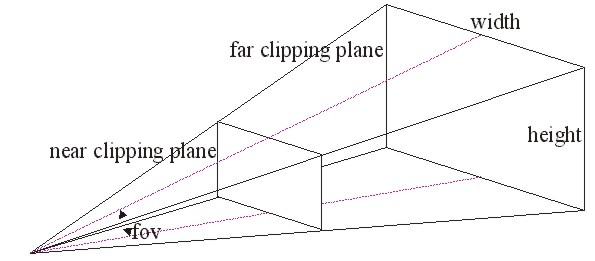
\includegraphics[width=0.9\linewidth]{img/clippingplane.jpg}
\caption{Perspective (Figure from \citep{clippingplane}).}
\label{fig:clippingplane}
\end{figure}
Inside the frustum is where you should draw, if you try to draw outside the bounds of the frustum, then nothing will be drawn and it will not consume resources. When setting up the game perspective we provide \ac{opengles} with the current aspect ratio of the screen, a field of view angle (denoted 'fov' in \autoref{fig:clippingplane}), and the depth of the near and far clipping planes. The width and height increases in size when we go deeper into the perspective, but the field of view angle always spans relative to the height of the screen. The width is always relative to the aspect ratio. This means that if we draw a square at a specific coordinate in the perspective, then the square will always have the same percent of space above and below it on the screen, but the space to the right and to the left of the square changes according to the aspect ratio of the screen.

The coordinate $(0, 0, 0)$ is where the perspective starts, or you could say it is where we are looking from. If you translate into the depth of the frustum e.g. $(0, 0, 50)$, then you are at the center of the perspective/screen.

The tablet has a resolution of $1280 \times 800$, but since it always displays a system bar with back-button, notifications, etc. we only have $1280 \times 752$ pixels of the screen available. All the graphics created for the game was made on a canvas with the same size as what we have available. In order to draw the graphics on the tablet screen we have to find the depth where the width and height in the frustum are the same as our screen size $1280 \times 752$.
\begin{figure}[H]
\centering
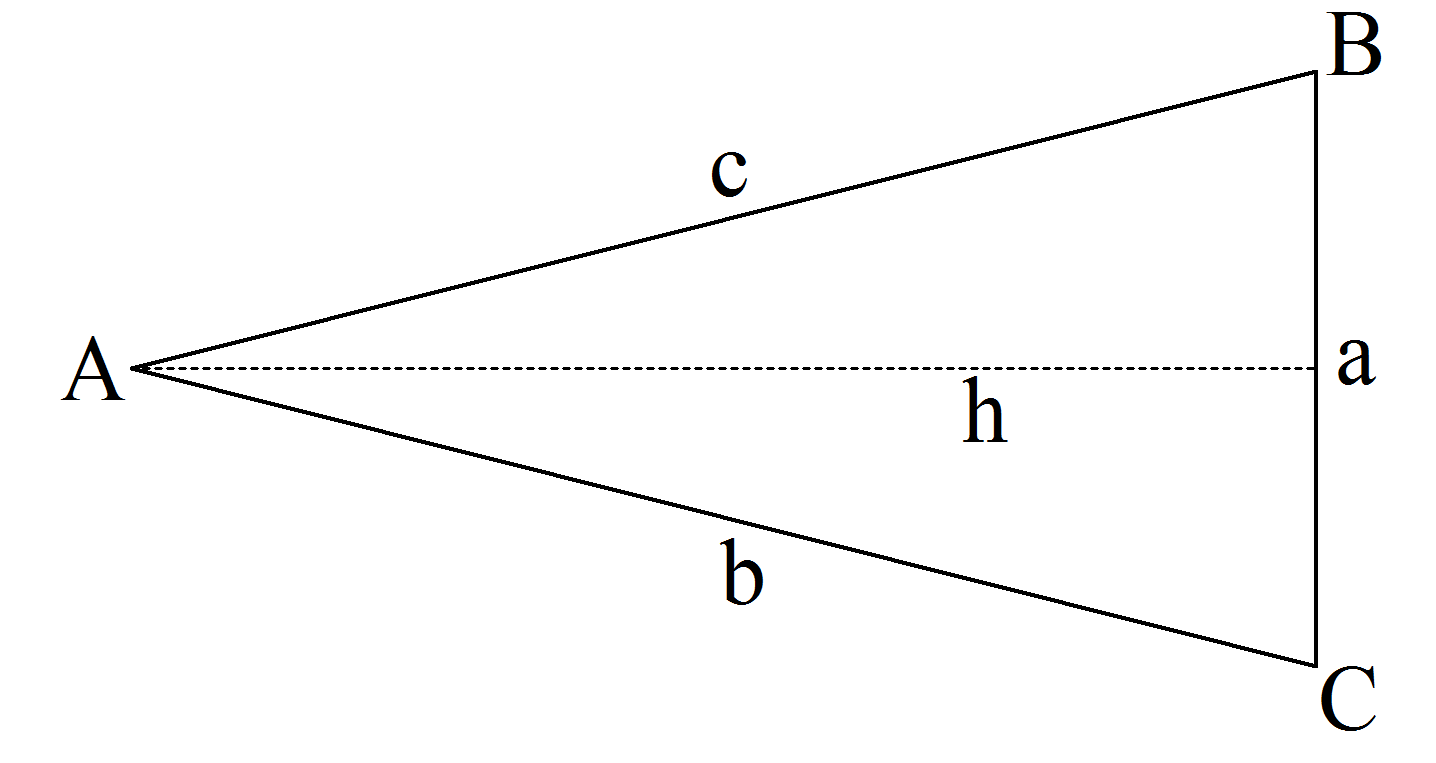
\includegraphics[width=0.5\linewidth]{img/trekant.png}
\caption{Perspective seen from the side.}
\label{fig:frustumside}
\end{figure}
\autoref{fig:frustumside} shows the perspective seen from the side, we want to find the height $h$ (depth) of the triangle when $a$ is the same size as our tablet $a = 752$. We have chosen a field of view angle to be $A = 45^{\circ}$. Since the angles $B$ and $C$ are the same size then
$$B = C = \frac{180^{\circ} - A}{2} = 67.5^{\circ}$$
Given $a$ and all the angles of the triangle, then $h$ is given by
$$h = \frac{a}{2} \times tan(B) = 907.7442$$
Now we have the depth of the perspective where one pixels of a texture corresponds to one pixels on the tablet screen. This will also make it possible to use pixels per millisecond as an actual unit of speed for our game.

%design chapter
\chapter{Design}
\todo{This Chapter describes the design of our application. It is split into two sections, one describing the design of our game and the other describing the design of menu.}
\section{Game}
In this section we will discuss and explain our thoughts about the game design, we will also comment on the feedback given by our contact person. Finally we will show the result of the game design.
\subsection{Game Idea/Description}
%Skriv hvordan spillet fungere
In \secref{processweek2} it is explained how Tove's version of the exercise work. We intent keep the same principles of Tove's exercise.
\subsubsection*{Game objects}
\begin{description}
\item[Pictogram] Is a object which contains a picture and is draggable.
\item[Train Station] Is a station where the train stops, and allows the child to drag and drop pictograms onto the station. Each station has a picture indicating the category of the station. The category of the station describes the pictograms that should be dropped onto the station.  

\item[Flute] Is a button that the child can press if they think that the correct pictograms have been dropped onto the station. If however the child have made a mistake and dropped a pictogram not belonging to the station's category, then the train would not start. The flute was added by Tove's request.

\item[Train and wagons] Is a vehicle that drives to each station, carrying pictograms in its wagons.

\item[Landscape sequence] Is a sequence of hills, trees, cow, and skies. The landscape sequence is placed between each stations, and creates the illusion that the train is driving to the next station.
\item[Train depot] When the train is driving from the last Train station, the train will drive into the a train depot to indicate the the game is over. The train depot was added by Tove's request.
\end{description}

\subsubsection*{Game Flow}
\todo{this section describes the flow of the game}
Our game starts by the child must drag the pictograms off the start Train station and drop them onto the train, the start station is special since it does not have a category. The start station is to help the child understand how to move pictures with drag and drop. When the child have moved all the pictures onto the train, it is allowed to drive through a landscape sequence, until it reaches the first train station.
The Train station has a category, which could be a picture of animals. It is now up to the child to drag all the animals off the train onto the station, so the train can continue. If all the right pictograms is on the station, the train will drive onto the next station. When all the pictograms is off the train the game will end.

\subsection{Game Prototype}
\todo{explain the prototype, and the what Tove liked, and would like add or change}
%vis billedet af prototypen, beskriv hvad Tove godt kunne lide, og hvad der kunne ændres, samt tilføjelser. (fløjten, ingen musik, no fancy colors on objects)
\begin{figure}[H]
\centering
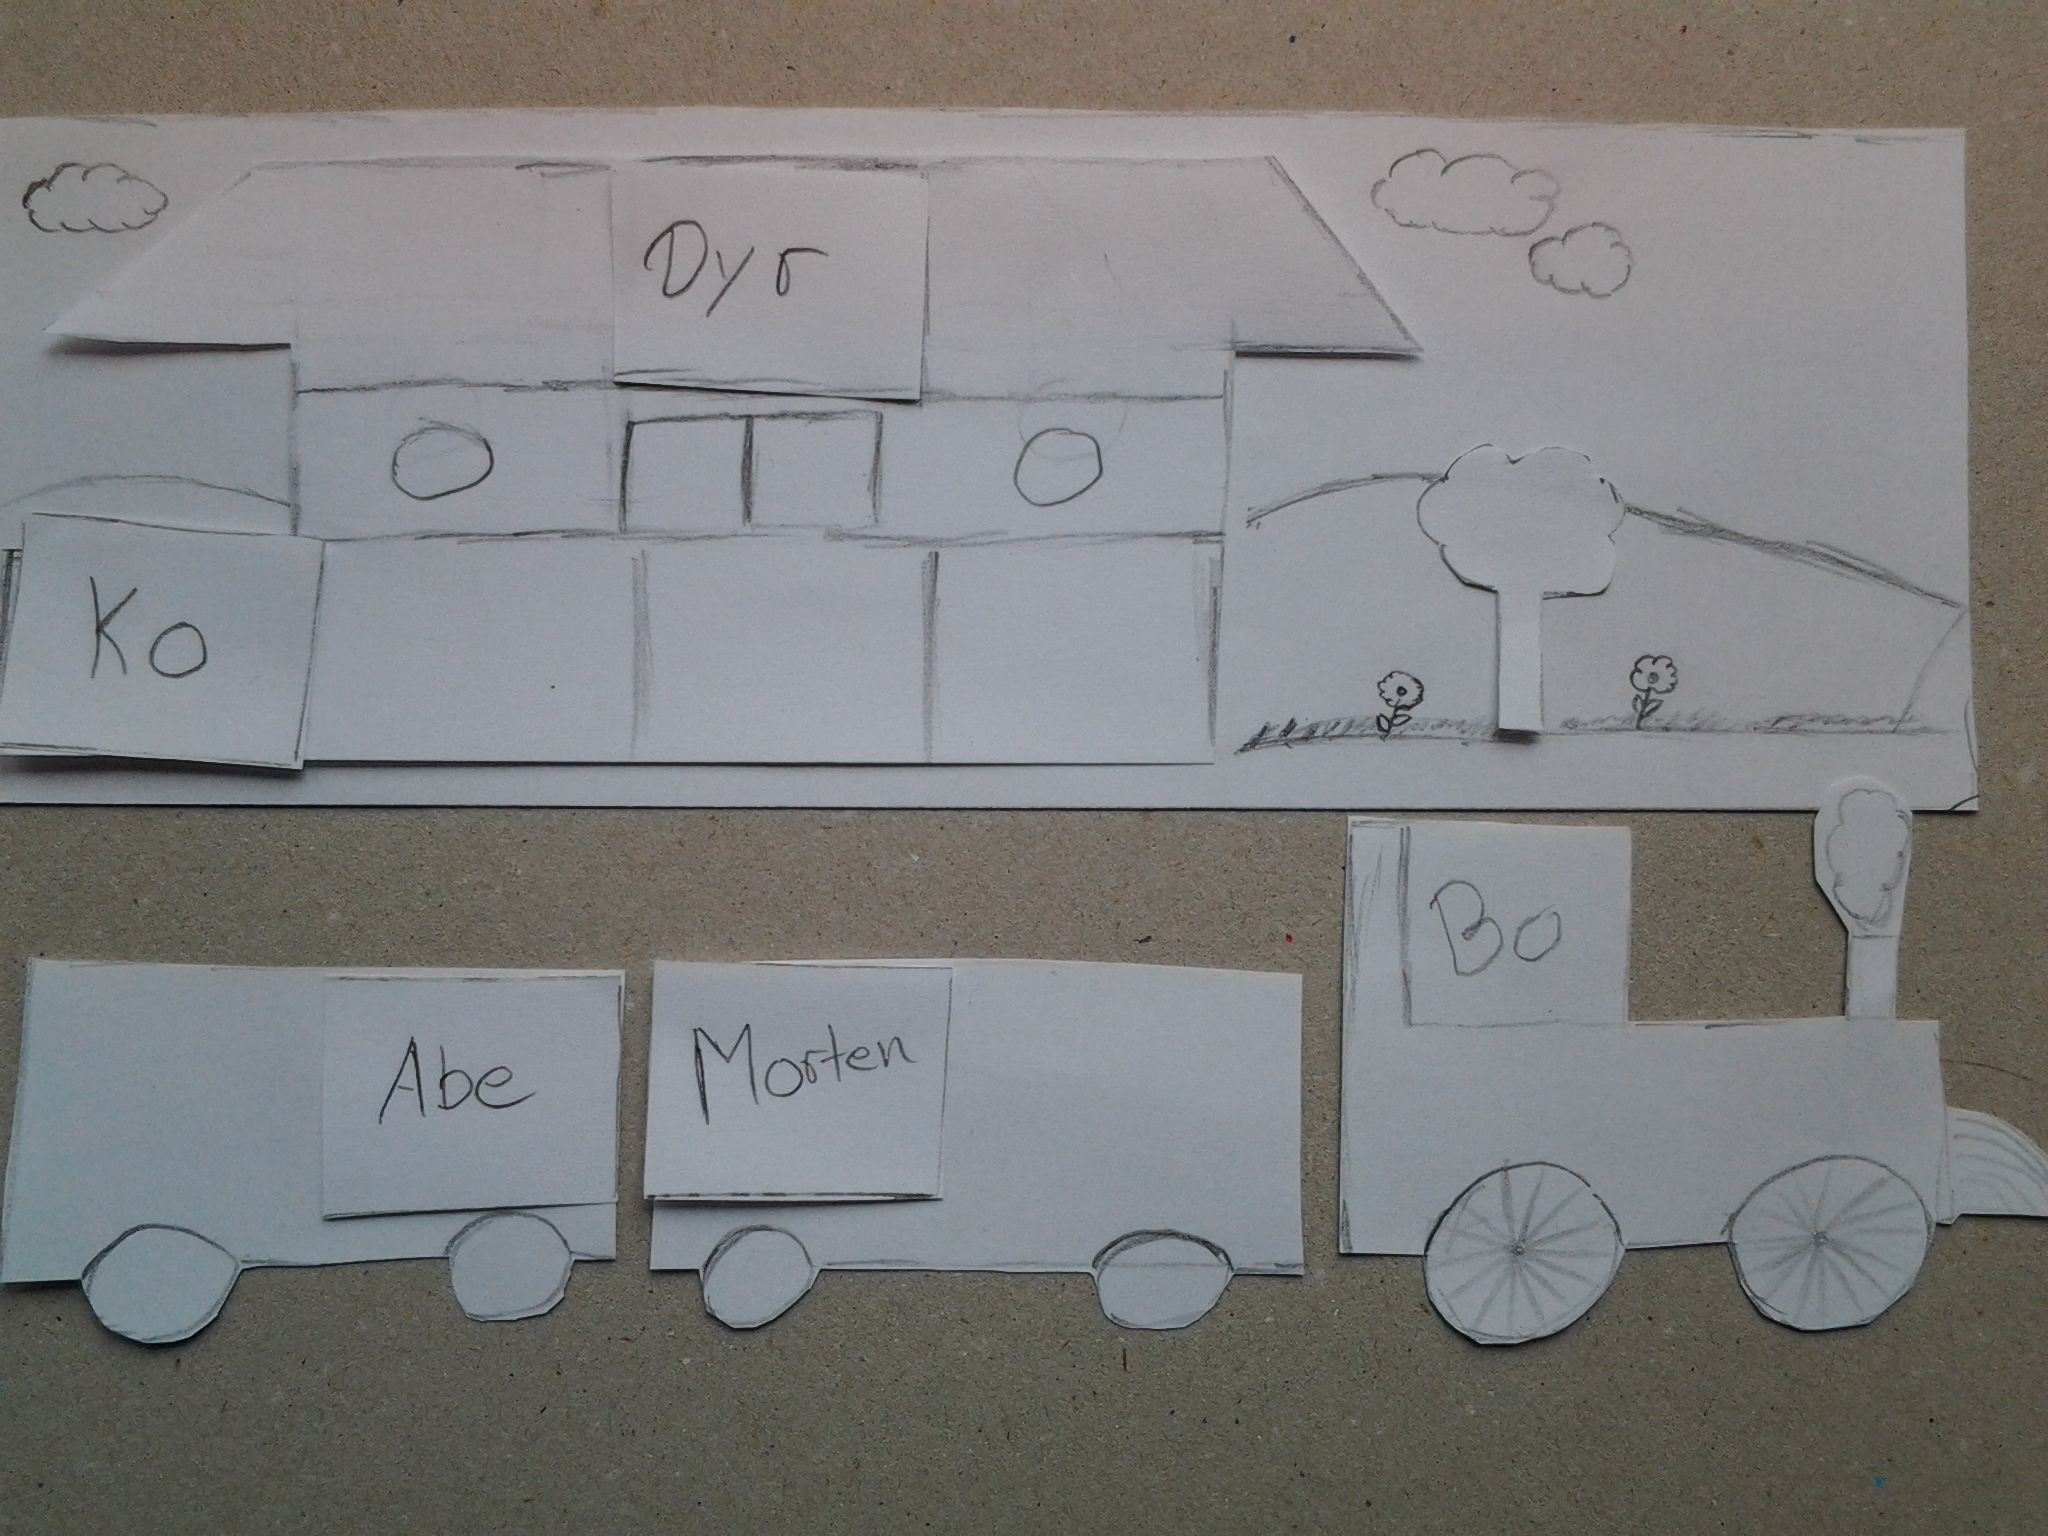
\includegraphics[width=0.9\linewidth]{img/screenshots/prototype1.jpg}%0.1 margin
\caption{The paper prototype}
\label{fig:paperprototype}
\end{figure}
\autoref{fig:paperprototype} shows the paper prototype we showed Tove at our first meeting, in which we explained our game idea. She liked the idea and the interface, although she would like to see a button that checks if the correct pictograms is off the train, if all pictograms is off, the train should start. She also mentioned that the game should have ending, she suggested that the train could drive into a train depot. The game should not contain many colors and sounds, since this would cause visual and audible noise for the child. The flute and train depot was added to the game idea after the meeting.


\subsection{Game Interface}


\label{designgameinterface}
\todo{describe the final result, show off a station and the entire game with one station.}
\begin{figure}[H]
\centering
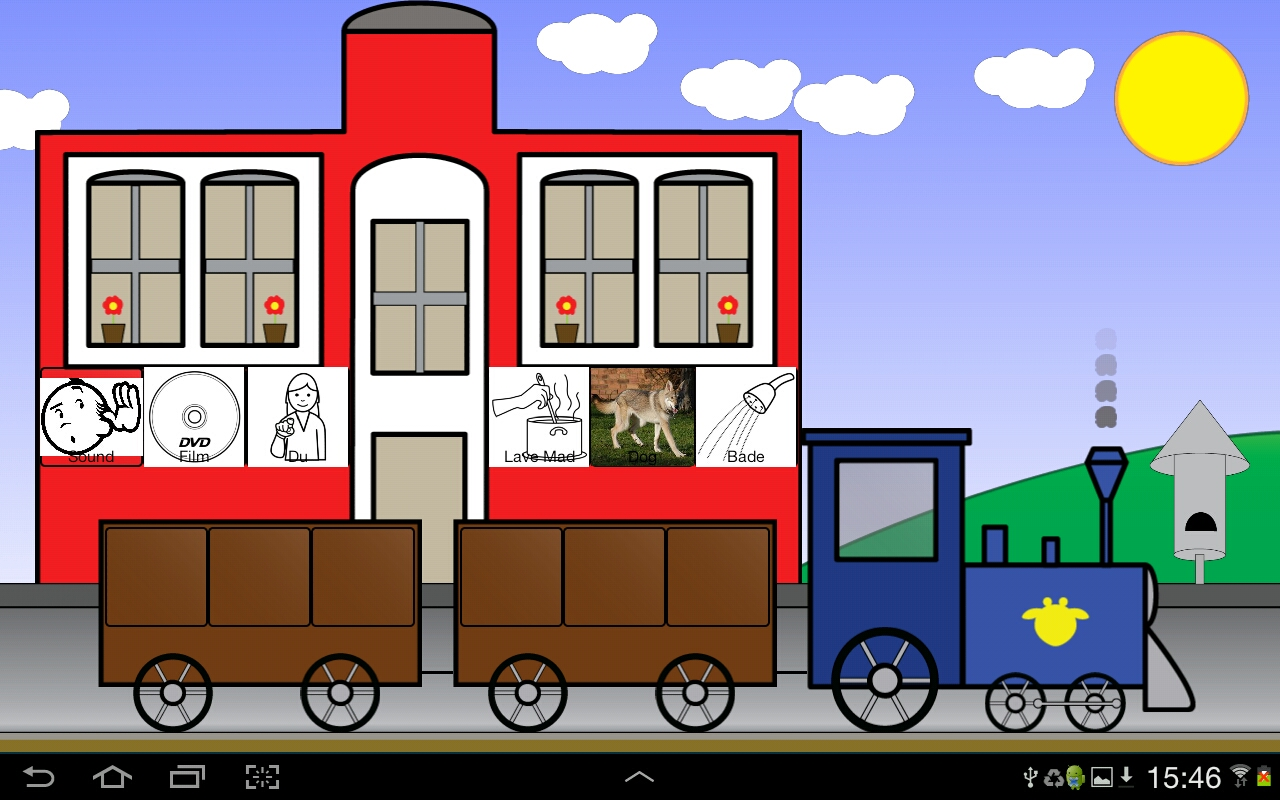
\includegraphics[width=0.9\linewidth]{img/screenshots/gamedesign1.jpg}%0.1 margin
\caption{The final result}
\label{fig:finalresult}
\end{figure}
During the project we sent screen shots of the game interface to Tove, to confirm that we were on the right track. For the most part she had not much to add, only small graphical adjustments to stations. 
In order to mimic Tove's version of the exercise we had to make the game customizable, we had to menu where Tove was able to customize the pictograms and the category for each station, the functionality is explained later in \secref{designmenu}. To prevent that the game is not the same every time we added random elements to the game, e.g. the order of stations, the hills in the landscape sequence, the decorative objects(cow, trees, skies) are also random placed.
%vis det endelig resultat, samt de ting som ikke noget at blive tilføjet.(Traindriver, click and autosnap, lyd på pictogrammer)

\chapter{Design}

\todo{This Chapter describes the design of our application. It is split into two sections, one describing the design of our game and the other describing the design of menu.}

\section{Game}
\todo{This section describes the design choices made in our game.}


\section{Menu}
\todo{This section describes the design choices made when creating our menu.}

\subsection{Flow}
To show the functionalities of the menu, the natural flow will be shown in this section.
\begin{figure}[H]
\centering
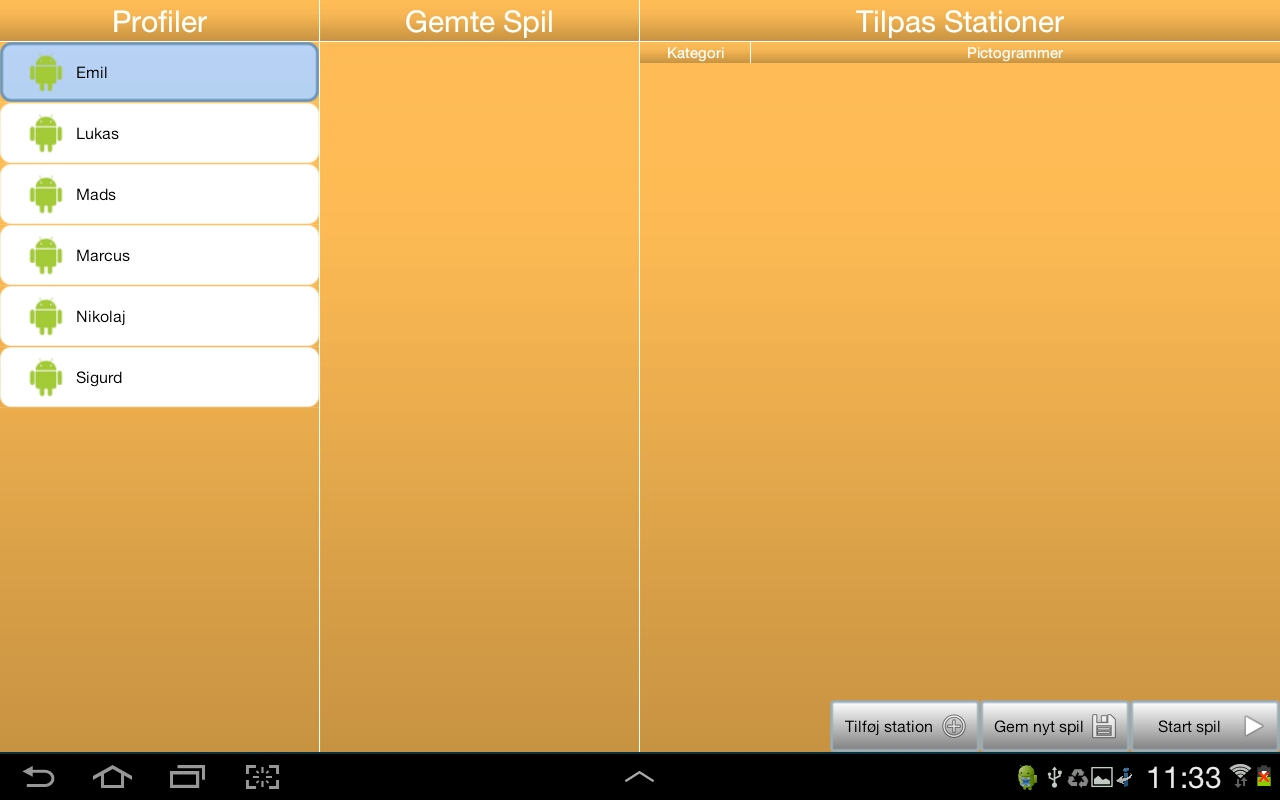
\includegraphics[width=0.9\linewidth]{img/screenshots/profile_flow_1.jpg}%0.1 margin
\caption{Profile flow 1}
\label{fig:profile_flow_1}
\end{figure}
\ref{fig:profile_flow_1} shows the general design of the menu. The overall color theme (Orange in this example) can be changed from the Launcher. The menu is divided into three parts; profiles, saved games, and game customisation. When the application is launched the menu will appear and the profile list will be populated with the children associated to the current guardian. In this example "Emil" has been chosen, but there are no saved games related to that child, yet.
We will now continue to push the "Tilføj station" (Add station) button three times.

\begin{figure}[H]
\centering
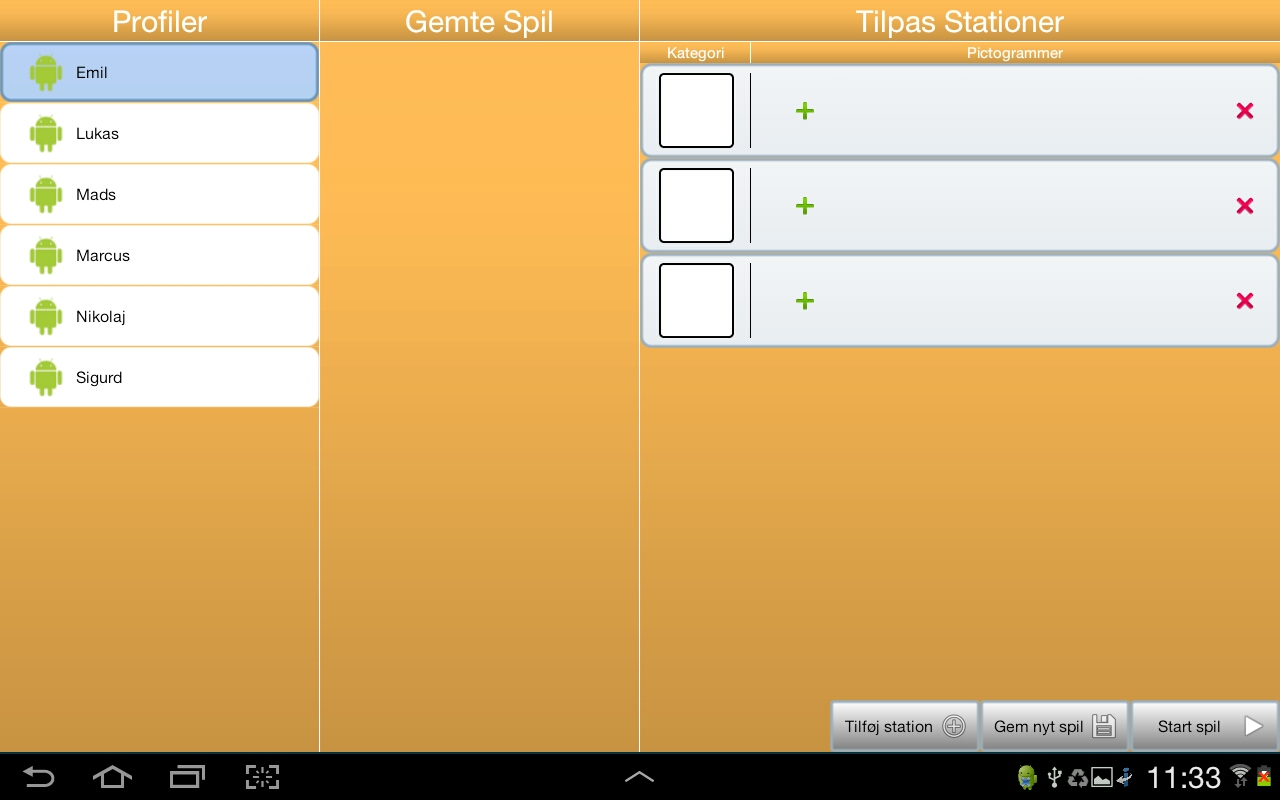
\includegraphics[width=0.9\linewidth]{img/screenshots/profile_flow_2.jpg}%0.1 margin
\caption{Profile flow 2}
\label{fig:profile_flow_2}
\end{figure}

The game customisation part of the menu has now been populated with three elements, each representing a station. An element/station consists of three buttons:
\begin{itemize}
\item \textbf{Add category:} Pressing the category pictogram will allow you to choose a different one. It is blank on default to show that no category has been selected.
\item \textbf{Add pictograms:} Pressing the green "+" will allow you to select the pictograms you want to be associated to the category.
\item \textbf{Delete station:} Pressing the red "x" will delete the station.
\end{itemize}
We will now continue to select a category for the first station by pressing the add category button.

\begin{figure}[H]
\centering
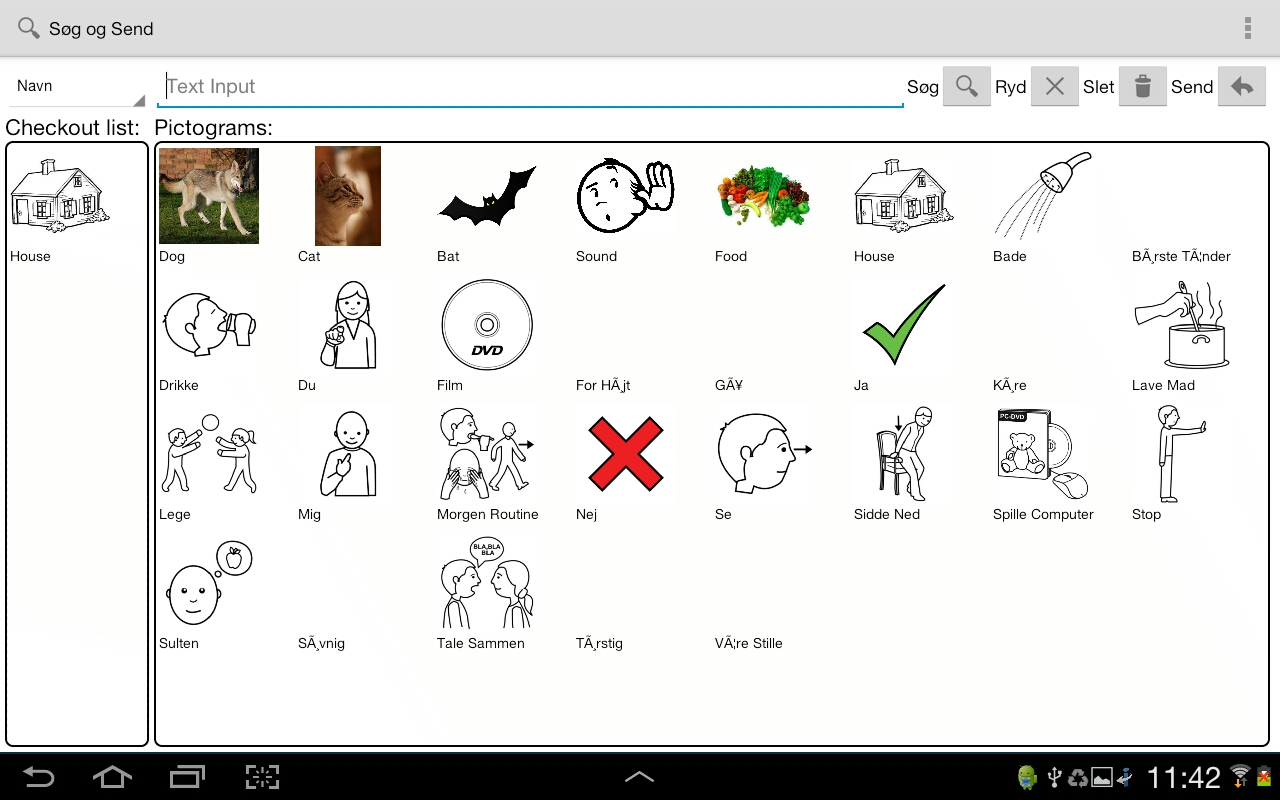
\includegraphics[width=0.9\linewidth]{img/screenshots/profile_flow_3.jpg}%0.1 margin
\caption{Profile flow 3}
\label{fig:profile_flow_3}
\end{figure}

\ref{fig:profile_flow_3} shows that CAT \todo{Acronym for CAT, go!} opens to allow you to select a pictogram to use for the category.
The pictogram "House" has been selected in this example, and we will now continue to press the "Send" button. This will send the pictogram back to the menu.

\begin{figure}[H]
\centering
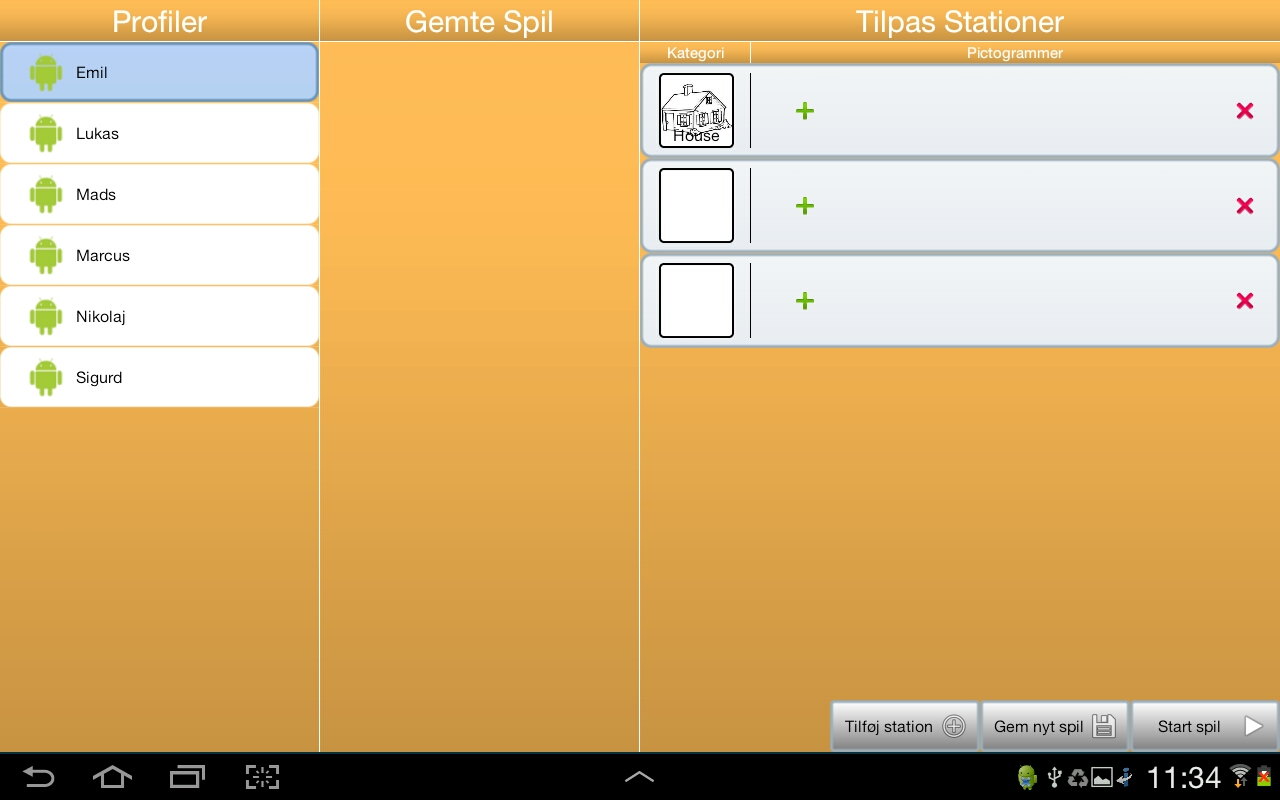
\includegraphics[width=0.9\linewidth]{img/screenshots/profile_flow_4.jpg}%0.1 margin
\caption{Profile flow 4}
\label{fig:profile_flow_4}
\end{figure}

It can now be seen in \ref{fig:profile_flow_4} that the pictogram we selected before has been set as the category for the first station. We will now press the green "+" to add the pictograms we want associated with this category.

\begin{figure}[H]
\centering
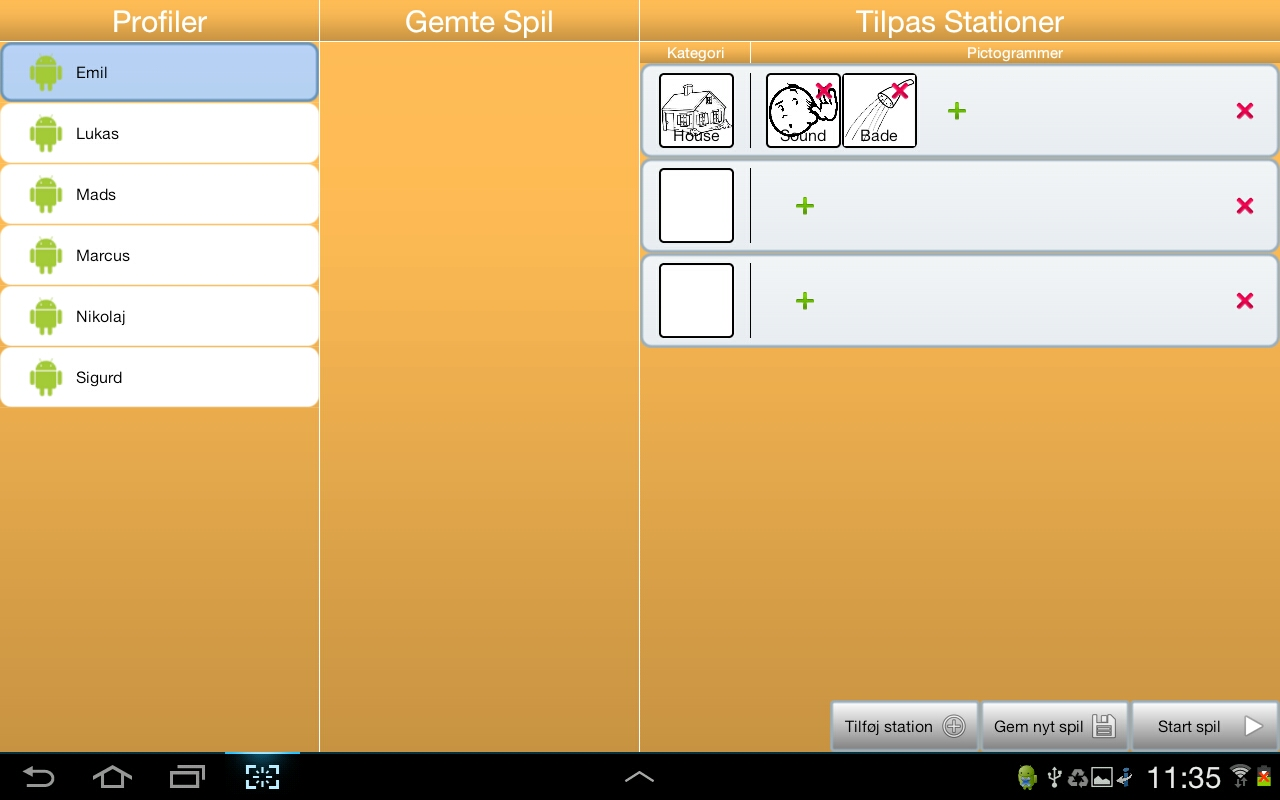
\includegraphics[width=0.9\linewidth]{img/screenshots/profile_flow_5.jpg}%0.1 margin
\caption{Profile flow 5}
\label{fig:profile_flow_5}
\end{figure}

It can be seen in \ref{fig:profile_flow_5} that two pictograms was selected, again via CAT. \todo{Acronym for CAT, go!} We will proceed to add categories and pictograms to the remaining stations, using the same method.

\begin{figure}[H]
\centering
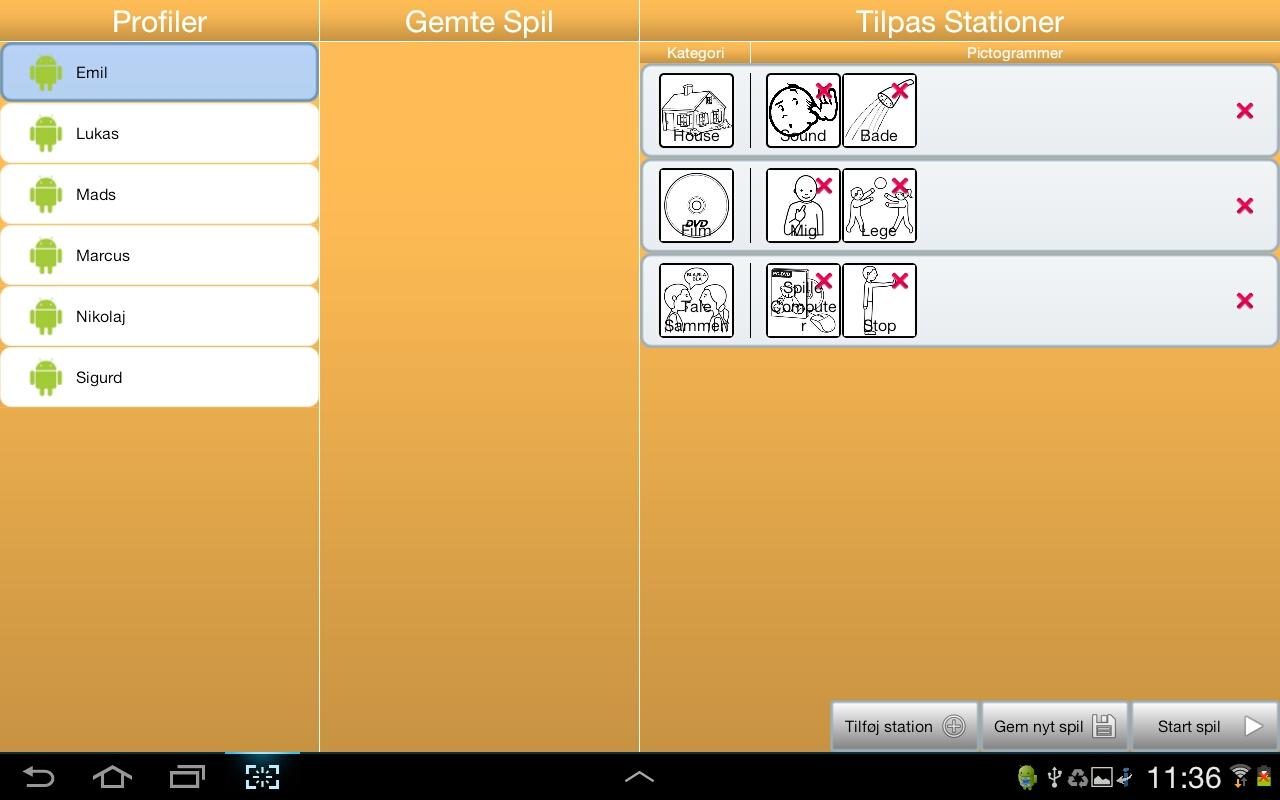
\includegraphics[width=0.9\linewidth]{img/screenshots/profile_flow_6.jpg}%0.1 margin
\caption{Profile flow 6}
\label{fig:profile_flow_6}
\end{figure}

\ref{fig:profile_flow_6} shows that the three stations have now been filled with pictograms. Note that the green "+" is gone, this is because we only allow a total of six pictograms. We will now press the "Gem nyt spil" button to save the game.

\begin{figure}[H]
\centering
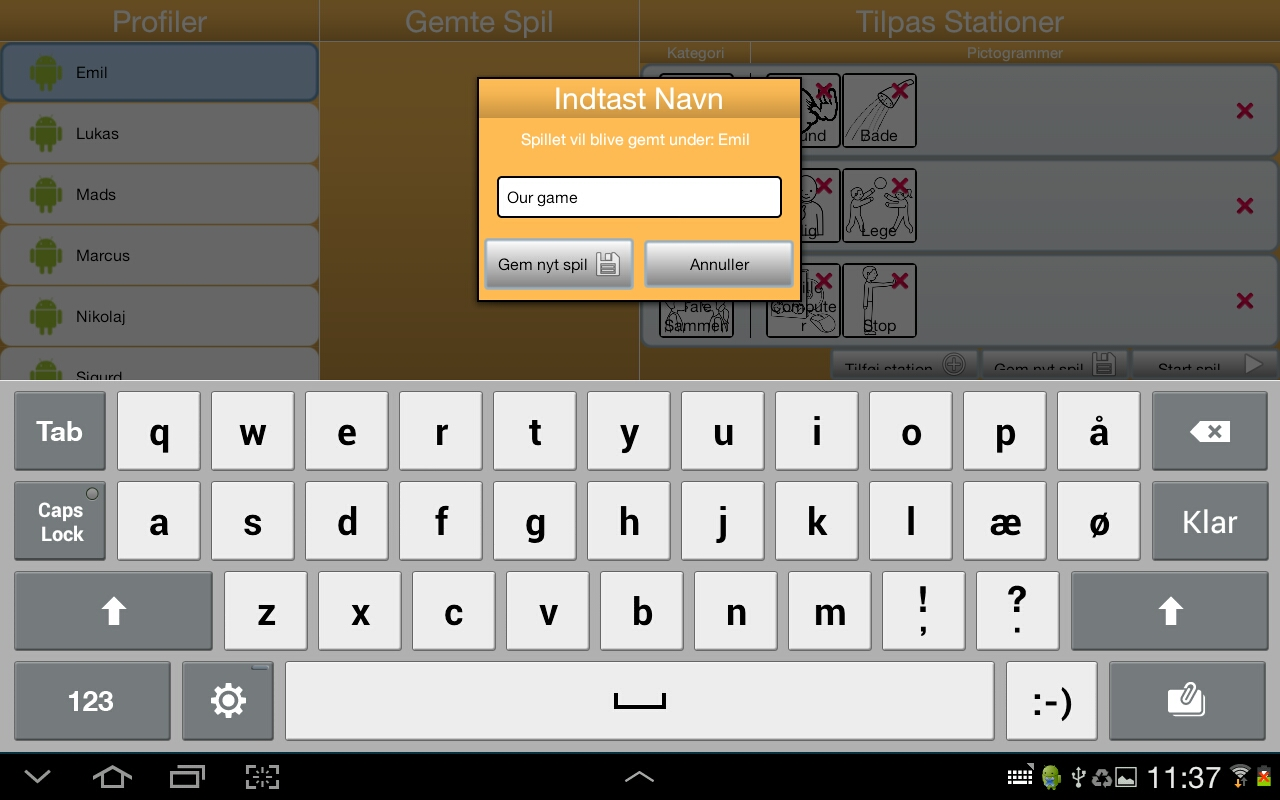
\includegraphics[width=0.9\linewidth]{img/screenshots/profile_flow_7.jpg}%0.1 margin
\caption{Profile flow 7}
\label{fig:profile_flow_7}
\end{figure}

\ref{fig:profile_flow_7} shows that a dialog appears when the save game button has been pressed. This dialog allows you to enter a name for your game and save it. We will call our game "Our game" and press "Gem nyt spil" which will save the game.

\begin{figure}[H]
\centering
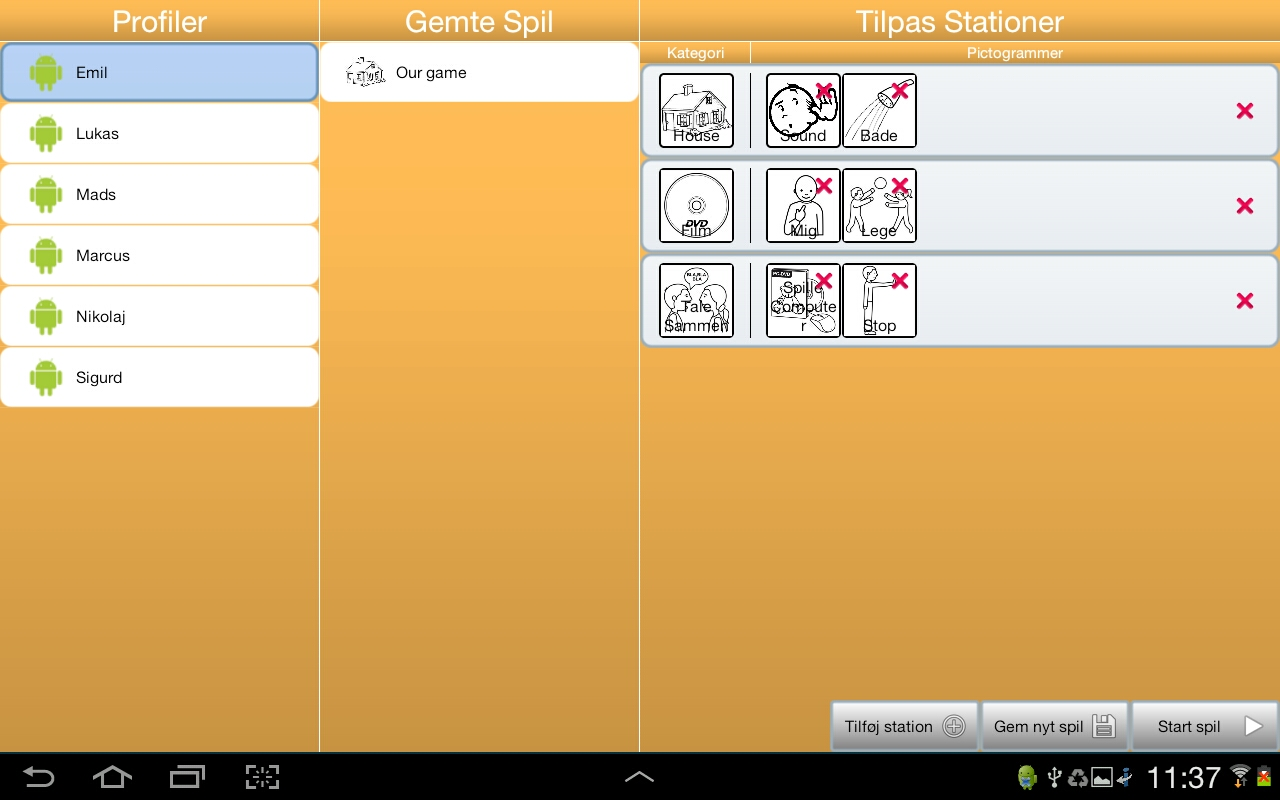
\includegraphics[width=0.9\linewidth]{img/screenshots/profile_flow_8.jpg}%0.1 margin
\caption{Profile flow 8}
\label{fig:profile_flow_8}
\end{figure}

The game configuration has now been saved, and is shown in the list of saved games. See \ref{fig:profile_flow_8}.\\
The newly saved game is linked to "Emil", and will show whenever he is selected.

\section{Game implementation}

This section describes how we have implemented the different elements of our game. It describes how we load and draw the texture for the train, how we have implemented the wheels and train smoke in order to create the illusion that the train is moving between the stations and how we randomly generate the background elements. .

\section{Train \& wagons}

The train and wagons are stationary textures on the tablet screen. \autoref{lst:loadtexture} shows how we load the texture for our train and wagons. 

\begin{lstlisting}[language=java,firstnumber=1,caption={Loading the texture for our train and wagons},label=lst:loadtexture] 
	// Initialize a train object and a wagon object
	private final Texture train = new Texture(1.0f, 1.0f);
	private final Texture wagon = new Texture(1.0f, 1.0f);

	//Load the textures
	this.wagon.loadTexture(R.drawable.texture_wagon, Texture.AspectRatio.BitmapOneToOne);
	this.train.loadTexture(R.drawable.texture_train, Texture.AspectRatio.BitmapOneToOne); 
\end{lstlisting}

\begin{description}
\item[Line 2 \& 3] Initialising the \textit{train} and \textit{wagon} objects 
\item[Line 6] This loads the \textit{wagon} texture, \textit{R.drawable.texture\_wagon} defines which texture gets loaded, which is this case is the wagon and \textit{Texture.AspectRatio.BitmapOneToOne} makes sure the texture keeps the original aspect ratio, as described in \secref{sec:renderables}.
\item[Line 7] This loads the \textit{train} texture, and the original aspect ratio is kept again. 
\end{description}

Now the texture is successfully loaded we have to place it on right location on the tablet screen. This is done using the coordinate system mentioned in\todo{ref til koordinatsystemet}. This is done as shown in \autoref{lst:addcoordinate}.

\begin{lstlisting}[language=java,firstnumber=1,caption={Placing the texture on the screen},label=lst:addcoordinate] 
	//Add coordnates to the renderables
	this.wagon.addCoordinate(-542.32f, -142.72f, GameData.FOREGROUND);
	this.wagon.addCoordinate(-187.45f, -142.72f, GameData.FOREGROUND);
	this.train.addCoordinate(160.42f, -52.37f, GameData.FOREGROUND);
\end{lstlisting}

\begin{description}
\item[Line 2\& 3] Since we have chosen to have two wagons on our train, we have to have two wagon objects, with their own coordinate. The coordinates are based on the coordinate system mentioned in \todo{ref til koordinatesystem}. \textit{GameData.Foreground} determines where in the clipping plane the objects are placed. 
\item[Line 4] Adds a coordinate for the placement of the \textit{train}.
\end{description}

Now the textures have been loaded and given coordinates, they are ready to be drawn. This is done as shown in \autoref{lst:drawtexture}

\begin{lstlisting}[language=java,firstnumber=1,caption={Drawing the texture on the screen},label=lst:drawtexture] 
	//Drawing the textures
	super.translateAndDraw(this.wagon);
	super.translateAndDraw(this.train);
\end{lstlisting}

\begin{description}
\item[Line 1 \& 2] This draws the \textit{wagon} and \textit{train} objects. The \textit{translateAndDraw} method is explained in \todo{Ref til afsnit on translateAndDraw}
\end{description}

\subsection{Wheels \& train smoke}

To create the illusion that the train is moving, we had to make wheels rotate in order to make it look like it was actually driving. 

The wheels are loaded and given a coordinate in the same way as the train that was just explained.

The difference comes when the wheels are drawn, we have to rotate the wheels so that it looks like the train moves, this is done by calculating the rotation using the function shown in \autoref{calcrotate}.

\begin{lstlisting}[language=java,firstnumber=1,caption={Rotating and drawing the wheels},label=lst:calcrotate]
    private float[] rotation = { 0f, 0f, 0f }; // rotation number for each wheel size
    private final double[] wheelDiameter = {
            106.39f, // large wheel
            78.71f,  // medium wheel
            60.8f    // small wheel
    };

    private final float calculateRotation(int wheelIndex) {    
        double circumference = this.wheelDiameter[wheelIndex] * Math.PI;
        double degreePerPixel = 360.0 / circumference;
        this.rotation[wheelIndex] += (float) degreePerPixel * super.gameData.getPixelMovement();
        return this.rotation[wheelIndex];
    }
\end{lstlisting}

\begin{description}
\item[Line 1] This array has the rotation number for each wheel size
\item[Line 2-6] This array has the diameter in pixels for each wheel size. 
\item[Line 8] The function takes a wheelIndex as parameter, this is to determine which the wheel size that is being used for calculations. 
\item[Line 9] The wheel's circumference is being calculated.
\item[Line 10] Calculating the degreePerPixel by dividing 360 with the circumference
\item[Line 11 \& 12] Here the rotation for the specific wheel is calculated by taking the degreePerPixel we just found and multiplying it by the pixel movement. \textit{GameData.getPixelMovement} is explains in \todo{ref til section med getPixelMovement}. Please note that the rotation is not reset, it keeps getting added to, however is it is not necessary to reset it as the rotation will not reach an overflow.
\item[Line 13] The specific wheel's rotation is returned. 
\end{description}

This function is called each time a wheel is drawn. This is done by using \textit{translateRotateAndDraw} as can be seen in \autoref{lst:rotatewheels}

\begin{lstlisting}[language=java,firstnumber=1,caption={Rotating and drawing the wheels},label=lst:rotatewheels]
	// Rotate and draw the wheels
super.translateRotateAndDraw(this.calculateRotation(this.mediumWheelIndex), this.mediumWheel);
super.translateRotateAndDraw(this.calculateRotation(this.largeWheelIndex), this.largeWheel);
super.translateRotateAndDraw(this.calculateRotation(this.smallWheelIndex), this.smallWheel);
\end{lstlisting}

\begin{description}
\item[Line 2-4] Each time a wheell has to be drawn, \textit{calculateRotation} with the specific wheelIndex as parameter and the rotation is calculated. The wheel is rotated and then drawn. 
\end{description}

\subsection{Station}

\subsection{Hills, trees, cows and clouds}

\chapter{Perspective}
\chapter{Perspective}
\todo{This Chapter describes some of the assignments our group have had throughout this multi-project.}
\textbf{STIKORD:}\\\\
\begin{itemize}
\item Reduceres drag listener på pictogrammerne (de ryster).
\item Game customisation optimisation. Listerne er langsomme.
\item Pictogrammer kun i opengl
\item Texture mipmaps
\item Solstråler.
\item Children list view skal være linear layout.
\item Mulighed for at overskrive spil.
\item Lyd på pictogrammer
\item Flere lydeffekter i spillet.
\item Databse \todo{Smid JSON queries ind her}
\item Setings menu, hvor du kan ændre farver og slå lyde til og fra osv. på ting i spillet.
\item Billede af det valgte barn som tog chauffør.
\item Gør det tydeligt at man kan slette ved at long-click
\item linearlayouts med pictogrammer forsvinder første gang man dragger.
\end{itemize}
\begin{lstlisting}[language=json,firstnumber=1,caption={JSON guery to read application data},label=lst:jsonread]
{
	"auth": {
		"session": SESSION_STRING
	},
	"action": "read",
	"data": {
		"type": "application",
		"view": "list",
		"ids": null
	}
}
\end{lstlisting} \todo{Skal muligvis skrives om, ved ikke om den er rigtig.}


\bookmarksetup{startatroot}% dette skulle stoppe part, så conclusion får indryk. Problemet i skrivende øjeblik er at chapters har samme indryk uafhængigt af parts
\addtocontents{toc}{\bigskip}%laver ekstra mellemrum

\chapter{Conclusion}
Our application was developed as a part of the GIRAF project 2013, a multi-project consisting of eight project groups, each with their own sub-project. Our focus in this project was to develop a game for GIRAF. 

The problem definition in \chapref{chap:intro} states:

\begin{quote}
\textit{"In what ways can we aid the pedagogues in their work with children with autism, by digitalizing a physical exercise onto an Android tablet?"} 
\end{quote}
The exercise we chose was an exercise that our contact person, Tove Søby, had presented during the first week of the project. The child had to place pictograms onto a train and unload them at the correct stations, this already allowed for great customization but required a lot of work from Tove Søby, so it was an ideal exercise for us to try and implement this on the Android platform. 

The main focus with our application was to make it customizable for the guardian, so that they easily can create new and different games for each child. 

We achieved this by creating a menu using LinearLayouts so they are possible to edit on runtime. The guardian is able to choose a specific child from the list and start creating a new game for that child. Using \ac{cat} they are able to choose the pictogram they want as category for each station and what pictograms they want associated with each station. This allows for customization with very limited effort from their side, which is what we wanted to achieve. 

The different graphical elements in the graphical side of the application is drawn in vector graphics, this makes it possible to resize the graphics in the future without a loss of quality. 

We have also implemented a whistle sound when the train starts driving and different random elements that can occur throughout the game, such as cows and trees on the hills in the background. This was done to create an element of surprise, which is something Tove Søby mentioned the children really liked.

Throughout the project we have communicated with Tove Søby for feedback and ideas and we have shown her and had her try out the application, however we do not have any official usability tests to document that our application is satisfactory, but we have managed to develop an application to aid the pedagogues in their work with autistic children, which was our goal for this project. 
\label{chap:conclusion}

\chapter{Future Work}
Unfortunately due to time limitations we have not been able to implement all the features that our contact person suggested. This Chapter describes some of the improvements that could be made on our application.

\textbf{STIKORD:}\\\\
\begin{description}
\item[The sun] The sun should have visible sunbeams, making it shine. 
\item[Overwrite games] At the moment it is not possible to overwrite an old game, each time you click the "Gem Spil" button, you save a new instance of a game even if you have changed an old game. It should be possible to overwrite existing games in order to make it easier for the user to edit and update them.
\item[Sounds on pictogram] The pictograms should have sounds, this could either be when you move them around or then you press them. 
\item[Sound effects in game] More sound effects in the game when the train is driving, such as the cow mooing or the wind blowing. 
\item[Customizable colors] All colors in the game are pre-determined right now. A settings menu where it is possible to change the color of items in the game, for example the color of the train and mute the different sounds could be possible in order to make it more customizable for the guardian.  
\item[Child as train driver] Every child has an avatar picture, it could be funny to have the child's avatar as the train driver. 
\item[Make it clear how to delete a game] It is possible to delete saved games by performing a long click, however this is not mentioned any where. Perhaps a little information button somewhere that explains this could be a good idea. 
\item[Greater variation of background features] The selection of background features is very limited, it can only be cows or trees. A greater selection of items could be implemented, perhaps to include planes, different kinds of animals or even humans. It should still be kept simple, but it would create a greater variation in the background. 
\item[Complete a station in one go] At the moment when creating new stations in the menu section, the user has to click the blank category box, open the PictoSearch, choose one category pictogram and click the "Send" button, then click the green plus and choose which pictograms to associate with the station.

An easier way for this could be to allow the user to click the blank category box and open PictoSearch and then allow them to choose up to seven pictograms, where the first pictogram would count as the category and the rest would be the pictograms associated with this specific station.
\item[Changing weather] One of the suggestions made by our contact person was that the weather could change while the train moved from one station to another, for example the sun could shine from the first to the second station and it could rain or snow from the second to the third station. 
\item Linearlayouts med pictogrammer forsvinder første gang man dragger.
\item Reduceres drag listener på pictogrammerne (de ryster).
\item Database \todo{Smid JSON queries ind her} 
\begin{lstlisting}[language=json,firstnumber=1,caption={JSON guery to read application data},label=lst:jsonread]
{
	"auth": {
		"session": SESSION_STRING
	},
	"action": "read",
	"data": {
		"type": "application",
		"view": "list",
		"ids": null
	}
}
\end{lstlisting} \todo{Skal muligvis skrives om, ved ikke om den er rigtig.}

\item Game customisation optimisation. Listerne er langsomme.
\item Pictogrammer kun i opengl
\item Texture mipmaps
\item Children list view skal være linear layout.


\end{description}


\begin{appendices}
\label{appendixStart}

\label{appendixEnd}
\end{appendices}
\newpage

\listoffigures

\newpage

\listoftables

\newpage

\lstlistoflistings

% Afslut med bibliografien. Bibliografien har mærkelige sidetal og side reference. Fixed med cleardoublepage og phantomsection
\cleardoublepage
\phantomsection
\label{chap:bib}% brugt i preface
\bibliography{bib/bibliografi}

\label{lastpage}% brugt i titelblad til total sidetal

\end{document}
